\documentclass[a4paper]{article}

% Packages
\usepackage[margin = 1 in]{geometry}
\usepackage{fancyhdr}
\usepackage{lastpage}
\usepackage{ctex}
\usepackage[utf8]{inputenc} % Required for inputting international characters
\usepackage[english]{babel}
\usepackage[T1]{fontenc} % Output font encoding for international characters
\usepackage[sfdefault]{ClearSans} % Use the Clear Sans font (sans serif)
\usepackage{graphicx}
\usepackage{caption}
\usepackage{subcaption}
\usepackage{float}
\usepackage{amsmath}
\usepackage{amsfonts}
\usepackage{enumitem}
\usepackage{hyperref}
\usepackage{titlesec}
\usepackage{lipsum}
\usepackage{geometry}
\usepackage{tocloft} 
\usepackage{tabularx}
\usepackage{pgfgantt}

\pagestyle{fancy}
% Formatting
\geometry{margin=1in}
\setlength{\parindent}{0pt}
\setlength{\parskip}{1em}
\renewcommand{\baselinestretch}{1.5}
\renewcommand{\cftsecleader}{\cftdotfill{\cftdotsep}}
\rhead{\thepage}

\begin{document}

%----------------------------------------------------------------------------------------
%	TITLE PAGE
%----------------------------------------------------------------------------------------

\begin{titlepage}
	
	\rule{\linewidth}{5pt}
	\raggedleft
	\fontsize{38pt}{50pt}\selectfont
    \textbf{\\Project Proposal\\}
    \fontsize{28pt}{60pt}\selectfont 
    for\\
    \fontsize{38pt}{60pt}\selectfont 
    \textbf{Mirror News Summarizer\\}
	
	\vfill % Space between the title box and author information
	
	%------------------------------------------------
	%	Author name and information
	%------------------------------------------------
	
	\parbox[t]{0.93\textwidth}{ % Box to inset this section slightly
		\raggedleft % Right align the text
		\large % Increase the font size
		{\bf Student Name:} Zijun Li\\
        {\bf Student ID:} 2272583\\
        {\bf Supervisor Name:} Jizheng Wan\\
        {\bf Project Category/Topic:} AI\\
	}
	
\end{titlepage}

\section{Project Aim:}

\begin{itemize}
    \item The goal is to develop `Mirror News Summarizer', an advanced platform that significantly enhances the user experience of consuming news online. It extracts content from selected news sites and, while maintaining a similar format reminiscent of the original website, eliminates advertisements and replaces full articles with succinct summaries to present on a mirror news platform. Furthermore, it offers a dedicated interface for tailored recommendations and a favorites section, ensuring personalized and engaging content for users. This system is meticulously designed to streamline the process of information acquisition, making news reading more efficient and user-friendly.
    \item {\bf Significance}: In today's digital age, users grapple with the deluge of information, often finding it challenging to decipher extensive content swiftly. The 'Mirror News Summarizer', with its mirror-style approach, elegantly addresses this by presenting concise news articles that encapsulate the essence of the original. This mirroring feature offers users a sense of familiarity and consistency, enhancing readability and reducing decision fatigue. By reducing the often dizzying array of design choices, it enhances readability and combats decision fatigue. Coupled with tailored recommendations and a favorites section, the platform not only ensures efficient news consumption but also elevates the user experience, crafting a more immersive and customized reading journey.
    \item {\bf Relevance to AI}: The `Mirror News Summarizer' leverages cutting-edge AI technologies and methodologies for several core functionalities:
    \subitem {\bf Summarization}: Employs Summary APIs, capitalizing on advanced NLP models like GPT (Generative Pre-trained Transformer), to generate precise and coherent news summaries. This AI-driven approach understands the context and extracts essential details, contributing to a succinct yet comprehensive summary.
    \subitem {\bf Recommendation System}: Integrates existing AI recommendation models that analyze user behavior, preferences, and interaction history to provide personalized news content, enhancing user engagement and satisfaction.
    \subitem {\bf Text Similarity Analysis}: Implements AI algorithms for text similarity checks to identify and eliminate duplicate content from different sources, presenting unique content to the users.
\end{itemize}

\section{Literature Review:}

In this chapter, we delve into an insightful comparison of some of the leading news recommendation and summarization platforms in the digital realm. 

\textbf{Inshorts}\cite{ref_web1} has positioned itself as a forerunner in the concise news space. Its backend, fortified by a rich tech stack of 22 products, from HTML5 to Google Analytics, ensures a seamless and responsive experience for its users.\cite{ref_web4} On the frontend, its minimalist yet impactful design delivers 60-word summaries that cut through the noise, making news consumption swift and straightforward. The user-centric mobile interface ensures quick access and readability, vital in today’s fast-paced world. However, its primary challenge remains its concentrated regional appeal, especially with India as its prime audience. Venturing into this space, the \textit{Mirror News Summarizer} encompasses advanced AI-driven personalization algorithms. Not only does it aggregate news, but it also tailors content based on individual preferences, enhancing global reach and user engagement.

\textbf{Feedly}\cite{ref_web2} is a master curator, with a technologically robust foundation that comprises 30 essential products, ensuring optimal content delivery from varied sources.\cite{ref_web5} Its interface is a blend of simplicity and categorization, allowing users to tailor their feeds based on interests. Yet, where it excels in aggregation, there's room for improvement in content condensation. As users demand both breadth and brevity, the \textit{Mirror News Summarizer} bridges this gap. By employing advanced algorithms, it not only collates content but also presents it in easily digestible chunks, ensuring that users receive depth without the associated reading time.

\textbf{Flipboard}\cite{ref_web3} is the epitome of visual storytelling in the digital news domain. Supported by an expansive tech stack and 182 website technologies, it offers a fluid, magazine-esque reading experience.\cite{ref_web6} The emphasis on visual elements, combined with its robust technological deployment, ensures users are always engaged. However, the focus on visuals sometimes comes at the cost of brevity. Recognizing this, the \textit{Mirror News Summarizer} marries visual appeal with content succinctness. The result is a platform that offers visual richness, but without compromising on the essence of the news.

Lastly, the \textit{Mirror News Summarizer} emerges as a holistic solution. It's not just about presenting news but doing so in a manner that resonates with the user's preferences and pace. Advanced AI algorithms, combined with user feedback loops, ensure that the platform learns and evolves with each user interaction. The addition of features like a 'favorites' section adds a layer of personal touch, ensuring users always have their preferred content at their fingertips.

\section{Project Objectives}

\begin{enumerate}
    \item \textbf{Interview \& User Persona Analysis}
    \subitem Understand the unique needs, preferences, and pain points of potential users of the Mirror News Summarizer through comprehensive interviews and persona analysis.
    % {\small\begin{itemize}
    %     \item \textbf{Zijun Li}
    %     \begin{itemize}
    %         \item Need for quick overviews of major news.
    %         \item Wants a platform that provides critical information rapidly.
    %         \item Prioritizes accuracy and reliability in news sources.
    %         \item Desires an interface free from ads or irrelevant content.
    %     \end{itemize}
    %     \item \textbf{Binghao Liu}
    %     \begin{itemize}
    %         \item Requires efficient and quick information access.
    %         \item Desires a platform that offers multimedia content for an enhanced learning experience.
    %         \item Values aesthetics and personalization in digital spaces, frequently customizing them.
    %         \item Hopes for an interface that can be modified according to his preferences.
    %         \item Expects concise yet comprehensive news summaries to stay informed without spending excessive time.
    %     \end{itemize}
    %     \item \textbf{Sabour}
    %     \begin{itemize}
    %         \item Needs personalized news recommendations.
    %         \item Desires bookmarking capabilities for ease of access.
    %         \item Values adaptive content that changes based on her reading habits and preferences.
    %         \item Expects a structured way to manage saved articles, including easy sorting and categorization.
    %     \end{itemize}
    % \end{itemize}}
    {\begin{itemize}
        \item \textbf{Feature List Compilation:}
        \begin{itemize}
            \item Quick News Summaries
            \item Personalized User Interface
            \item Aesthetic and User-Friendly Design
            \item Intelligent Content Filtering
            \item Distraction-Free Reading Mode
            \item Reliable News Sources Integration
        \end{itemize}
    \end{itemize}}
    \item \textbf{Agile Development Process}
    \begin{itemize}
        \item \textbf{MVP (Minimum Viable Product)}
        \begin{itemize}
            \item Develop a news summary tool that offers concise overviews of major news topics by mirroring a specific website and successfully implementing web scraping for that site.
            \item Implement a reliable and accurate news aggregation algorithm.
            \item Establish a basic recommendation system to curate news articles for individual users.
        \end{itemize}
        \item \textbf{Iterative Enhancements:}
        \begin{itemize}
            \item Personalized news recommendation engine that evolves based on users' reading habits.
            \item Bookmarking feature, allowing users to save and return to articles at their convenience.
            \item Ad-free and distraction-free user interface to enhance readability and user experience.
            \item Categorization and sorting options for saved articles, providing better organization.
        \end{itemize}
        \item \textbf{Feedback \& Iteration:}
        \begin{itemize}
            \item Continually gather feedback from the user personas (and broader user base) to refine and improve features.
            \item Prioritize feature developments based on both user feedback and technological advancements in the field.
        \end{itemize}
    \end{itemize}
    \item \textbf{Test \& Evaluation}
    \begin{itemize}
        \item \textbf{Continuous Integration (CI):}
        \begin{itemize}
            \item Implement CI tools to ensure code quality and to detect issues early.
            \item Regularly test new features in isolation before merging them with the main application.
        \end{itemize}
        \item \textbf{Continuous Deployment (CD):}
        \begin{itemize}
            \item Automated deployment of the application to a production environment after passing CI tests.
        \end{itemize}
        \item \textbf{User Acceptance Testing (UAT):}
        \begin{itemize}
            \item Before major releases, conduct UAT with real users to ensure the application meets their needs and expectations.
            \item Adjust features based on feedback from UAT.
        \end{itemize}
        \item \textbf{Debugging:}
        \begin{itemize}
            \item Regularly monitor application logs and user feedback to identify and fix bugs.
            \item Prioritize bugs based on their impact on user experience and application stability.
        \end{itemize}
    \end{itemize}
\end{enumerate}

\section{Project Deliverables}

\begin{enumerate}
    \item User-Centric News Access and Customization
        \begin{itemize}
            \item Develop a user authentication and login system, ensuring secure and consistent access to personalized news settings across different devices.
            \item Develop a user interface within the 'Mirror News Summarizer' that allows individuals to choose their preferred news sources and categories, enhancing personalized interaction.
            \item Implement a content filtration and retrieval system that curates and presents news from selected mirror news websites, optimizing the influx of information based on user preferences.
        \end{itemize}
    \item Enhanced Content Presentation
        \begin{itemize}
            \item Design an intuitive layout to display summarized news content, incorporating essential details like the headline, source, publication date, and core points, all within a user-friendly, visually appealing framework.
            \item Establish a mechanism for users to customize the news summary display, including aspects like theming (dark mode, font choices) and organization (list view, card view), further improving user experience and accessibility.
        \end{itemize}
    \item Intelligent Content Summarization and Duplication Check
        \begin{itemize}
            \item Execute an AI-driven process for dynamic news content summarization, ensuring that the essence and critical points of the full articles are cohesively maintained in the shortened version.
            \item Integrate a text similarity analysis feature that identifies and filters out repetitive news from different sources, thereby avoiding content redundancy and enhancing the quality of content presented to the user.
        \end{itemize}
    \item Adaptive Recommendation and Interaction System
        \begin{itemize}
            \item Construct a recommendation engine that analyses user interactions, preferences, and trending news to suggest relevant content, thereby personalizing the user's news feed and improving content relevancy.
            \item Develop interactive components within the platform, such as feedback options for summaries and bookmarking capabilities for preferred news articles, fostering user engagement and platform loyalty.
        \end{itemize}
    \item Voice Integration and Multilingual Support
        \begin{itemize}
            \item Integrate a text-to-speech feature, enabling users to listen to news summaries, thereby accommodating different user needs and enhancing accessibility.
            \item Incorporate a multilingual interface, allowing the platform to serve a broader demographic, catering to users from various linguistic backgrounds, and expanding the platform's reach.
        \end{itemize}
    \item User Engagement and Analytic Reports
        \begin{itemize}
            \item Implement a system for tracking user engagement metrics, preferences, and feedback, utilized for continuous improvement of the platform's features and user experience.
        \end{itemize}
\end{enumerate}

\section{Methodologies}

\begin{enumerate}
    \item {\bf User Authentication and Login}: Develop a secure user registration and login mechanism using technologies like JWT (JSON Web Tokens) and OAuth. This step ensures a protected, personalized space for each user and sets the foundation for subsequent personalized interactions.
    \item {\bf User Preferences and Customization Setup}: Initiate user interaction by offering a setup interface where they can select preferred news categories, sources, and UI/UX elements (e.g., dark mode, text size). This step personalizes the subsequent content curation.
    \item {\bf Content Aggregation and Filtration}: Utilize web scraping tools (like requests) and APIs to aggregate news content from various mirror websites selected by the user. This process includes filtering out ads and non-essential elements, focusing solely on the actual news content.
    \item {\bf AI-driven News Summarization}: Implement an AI model API to generate concise, coherent summaries of the aggregated news articles. This step requires maintaining the integrity and critical nuances of the original news content while reducing the length.
    \item {\bf Duplication and Redundancy Removal}: Apply text similarity algorithms to identify and eliminate duplicate content across multiple news sources, ensuring a unique, clutter-free user feed.
    \item {\bf Dynamic Content Presentation}:Display the summarized content to users in a structured, customizable UI, allowing for different viewing preferences (e.g., list view, card view). This stage involves frontend technologies like React for a responsive design.
    \item {\bf User-Interactive Recommendation System}: Integrate a recommendation system that tracks user engagement (clicks, reading time) and utilizes existing models to suggest relevant news, enhancing the personalization aspect of content delivery.
    \item {\bf User Feedback and Continuous Improvement}: Allow users to provide feedback on news summaries and recommendations, which the system will use for continuous learning and improvement. This iterative process is crucial for maintaining content relevance and accuracy.
    \item {\bf Text-to-Speech (TTS) and Multilingual Support Integration}:Incorporate TTS functionality for users to listen to summaries, enhancing accessibility, and convenience. Additionally, implement multilingual support to cater to a diverse user base.
    \item {\bf Backend Support and Data Management}: Use backend technologies like Flask for managing data transactions, user requests, and system responses, ensuring a seamless, efficient backend operation.
    \item {\bf Evaluation and User Testing}: Conduct comprehensive user testing to evaluate the system's performance, particularly the accuracy of news summaries, effectiveness of the recommendation engine, and overall user satisfaction. Collect feedback for future enhancements.
\end{enumerate}

\section{Project Plan}

% \begin{table}[h!]
%     \begin{tabularx}{\linewidth}{|c|c|X|}
%     \hline
%     Week       & Dates         & Tasks                                                                                                                              \\ \hline
%     Week 1-6   & 9.25 - 11.5   & \begin{tabular}[c]{@{}l@{}}- Make Mockup and Personas \\ - Write Proposal\end{tabular}                                              \\ \hline
%     Week 7-8   & 11.6 - 11.19  & \begin{tabular}[c]{@{}l@{}}- Initialize the frontend: Set up tools and frameworks\\ - Initialize the backend: Set up server and database\\ - Design a simple Interface prototype\end{tabular}                          \\ \hline
%     Week 9-10  & 11.20 - 12.3  & \begin{tabular}[c]{@{}l@{}}- Develop a Website crawler: Define sources and extractors\\ - Integrate Content Summarizer(API): Set up API calls and \\responses\end{tabular}                                   \\ \hline    
%     \end{tabularx}
% \end{table}

\begin{table}[h!]
    \begin{tabular}{|c|c|l|}
    \hline
    Week       & Dates         & Tasks                                                                                                                              \\ \hline
    Week 1-6   & 9.25 - 11.5   & \begin{tabular}[c]{@{}l@{}}- Make Mockup and Personas \\ - Write Proposal\end{tabular}                                              \\ \hline
    Week 7-8   & 11.6 - 11.19  & \begin{tabular}[c]{@{}l@{}}- Initialize the frontend: Set up tools and frameworks\\ - Initialize the backend: Set up server and database\\ - Design a simple Interface prototype\end{tabular}                          \\ \hline
    Week 9-10  & 11.20 - 12.3  & \begin{tabular}[c]{@{}l@{}}- Develop a Website crawler: Define sources and extractors\\ - Integrate Content Summarizer(API): Set up API calls and \\responses\end{tabular}                                   \\ \hline    
    Week 11-12 & 12.4 - 12.17  & \begin{tabular}[c]{@{}l@{}}- Implement Recommend System: Design algorithms and \\interfaces\\ - Develop a Repeat Content Checker: Set up detection algorithms\\ - Draft 50\% of the report: Define structure and content\end{tabular} \\ \hline
    Week 13-14 & 12.18 - 12.31 & \begin{tabular}[c]{@{}l@{}}- Set up a Feedback System: Design UI and backend handlers\\ - Optimize UI: Improve navigation menu, Redesign key pages \\ - Finish MVP(Minimum Viable Product) \end{tabular}                                                     \\ \hline
    Week 15-16 & 1.1 - 1.14    & \begin{tabular}[c]{@{}l@{}}- Implement Voice Integration: Choose voice API and integrate\\ - Add Multilanguage Support: Define languages and integrate \\translation APIs\\ - Implement CI/CD: Set up pipelines and deployment strategies\\ \end{tabular}        \\ \hline
    Week 17-18 & 1.15 - 1.28   & \begin{tabular}[c]{@{}l@{}}- Get feedback using UAT \\ - Draft GDPR policy: Define data collection and usage\\ - Create DPIA form: Define risk assessment criteria\\ - Draft 80\% of the report: Refine content and gather feedback\end{tabular}                                                                                                      \\ \hline
    Week 19-20 & 1.29 - 2.11   & \begin{tabular}[c]{@{}l@{}}- Debug the system: Set up testing environments and fix issues\\ - Adjust according to UAT\\ - Finalize and proofread the report\end{tabular}                    \\ \hline
    Week 21-22 & 2.12 - 2.25   & \begin{tabular}[c]{@{}l@{}}- Create app-demo: Showcase key features and functionalities\\ - Design a11y-demo: Highlight accessibility features and \\improvements\end{tabular}                                                                                                        \\ \hline
    \end{tabular}
\end{table}

\begin{figure}[H] %H为当前位置,!htb为忽略美学标准,htbp为浮动图形
	\centering %图片居中
	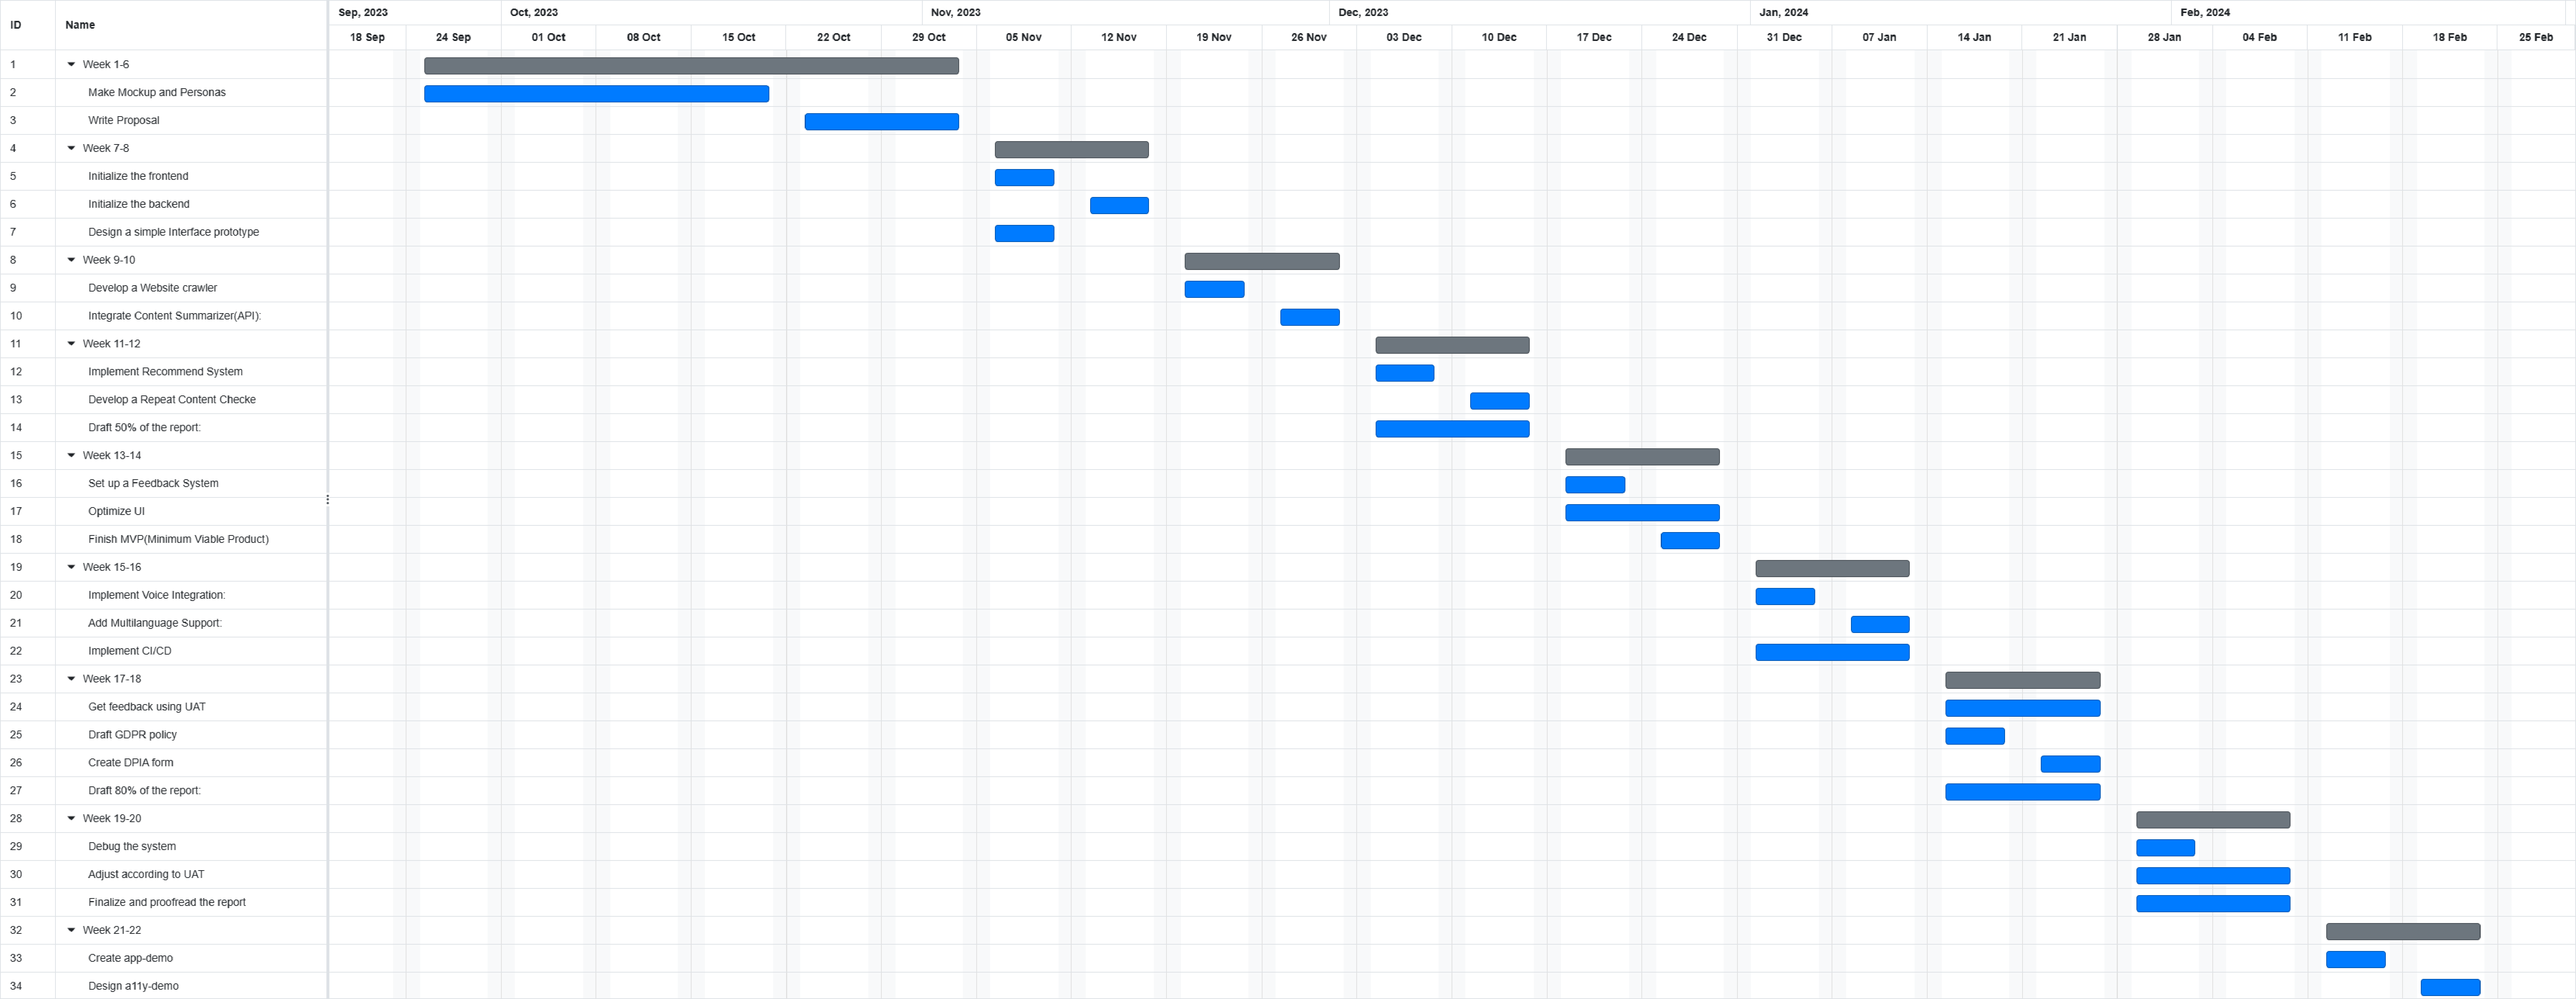
\includegraphics[width=1\textwidth]{./images/Online Gantt 20231101.pdf} %插入图片,[]中设置图片大小,{}中是图片文件名
	\label{Fig.Gantt} %用于文内引用的标签
\end{figure}

\section{Risks and contingency plan}

\begin{itemize}
    \item \textbf{Risk}: Web scraping tools often depend on the consistent structure of a webpage. If major news sites undergo a significant design overhaul, the scraping tools developed for the 'Mirror News Summarizer' might fail to aggregate content effectively.
    \subitem \textbf{Contingency}: Should our primary targeted news sources change their webpage structures, we plan to quickly adapt our scraping scripts. Furthermore, we'll set up periodic monitoring tools to check the efficiency of our scrapers and get alerts for potential failures.
    \item \textbf{Risk}: News websites frequently employ anti-scraping technologies and techniques to prevent automated bots from accessing their content. This can hinder the consistent inflow of news data to the platform.
    \subitem \textbf{Contingency}: In the event we encounter difficulties accessing content from a particular source, we'll pivot to integrate RSS feeds or official news APIs, which offer structured and consistent access to news articles.
    \item \textbf{Risk}: Third-party APIs often have usage limits or rate limits that could restrict the extent and frequency of operations, affecting the performance of our summarization system if the project scales up.
    \subitem \textbf{Contingency}: If we approach the API rate limits, our plan is to integrate caching mechanisms to store frequently accessed summaries. Additionally, we'll explore the possibility of incorporating other summarization algorithms or tools to diversify our backend and reduce dependency on a single API.
\end{itemize}

\section{Hardware/Software Resource}

\begin{enumerate}
    \item Hardware:
    \begin{itemize}
        \item RAM: 4 GB
        \item Storage: 50 GB
    \end{itemize}
    \item Software Requirements:
    \begin{itemize}
        \item OS: Windows
        \item Python 3.8 or later
        \item Text Editor or IDE: VS Code/PyCharm
        \item Browser: Google Chrome/Edge
        \item Database Management System: MySQL/PostgreSQL/SQLite
        \item Backend: Flask
        \item Frontend: React.js
        \item Web scraping tools: Beautiful Soup
        \item Summary API key: OpenAI API
        \item Version Control: Git
    \end{itemize}
\end{enumerate}

\section{Data}

\begin{itemize}
    \item The primary data for the project comprises news articles and content fetched from various online news websites through web scraping techniques.
    \item The data includes textual content, publication dates, author names, and other relevant metadata associated with each news article.
    \item User interaction data, such as reading preferences, feedback on summaries, and browsing history, will be collected through the platform to enhance the recommendation system.
    \item Ethical considerations and privacy compliance measures are in place for handling user data, with protocols established for secure data storage, retrieval, and processing.
\end{itemize}

\newpage

\begin{thebibliography}{}
    \bibitem{ref_web1}
    Inshorts. (n.d.). Retrieved from \url{https://www.inshorts.com/en/read}
    
    \bibitem{ref_web2}
    Feedly: Discover. (n.d.). Retrieved from \url{https://feedly.com/i/discover}
    
    \bibitem{ref_web3}
    Flipboard. (n.d.). Retrieved from \url{https://flipboard.com/}
    
    \bibitem{ref_web4}
    Inshorts - Technology. (n.d.). Crunchbase. Retrieved from \url{https://www.crunchbase.com/organization/news-in-shorts/technology}
    
    \bibitem{ref_web5}
    DevHD - Technology. (n.d.). Crunchbase. Retrieved from \url{https://www.crunchbase.com/organization/devhd/technology}
    
    \bibitem{ref_web6}
    Flipboard - Technology. (n.d.). Crunchbase. Retrieved from \url{https://www.crunchbase.com/organization/flipboard/technology}
\end{thebibliography}

\end{document}